\chapter{Wi-Fi}
\label{ch:wifi}
\textbf{Wi-Fi} is a family of wireless network protocols, based on the IEEE 802.11 standards (of which it constitutes a subset), which are commonly used for local area networking and Internet access. Wi‑Fi is a trademark of the non-profit \textbf{Wi-Fi Alliance}, which restricts the use of the term \textit{Wi-Fi Certified} to products that successfully complete interoperability certification testing. The Wi-Fi Alliance is not part of the IEEE, but it is an alliance of commercial providers (companies) that assembled together to promote this standard.

%----------------------------------------------------------------------------------------

\section{About the standards}
In order to make their standard, the Wi-Fi Alliance basically picked up parts of the 802.11 standards and declared them mandatory or optional. What happened is that what we see in 802.11b, 802.11g or 802.11n has been actually translated by the Wi-Fi Alliance into a set of rules that tells us which parts of the standard have to be implemented in order to be compliant with the Wi-Fi version (b/g/n and so on). The actual standard of each version contains everything inside, and it is only different from the other versions in the specifications regarding the mandatory and optional parts. Mind that in the standard we might also find things which are not part of a normal Wi-Fi implementation. Following is the list of Wi-Fi standards (as of fall 2020; missing letters are not missing, but have been omitted because the list would have been too long):

\begin{multicols}{3}
\begin{itemize}
    \item 802.11-1997
    \item 802.11a
    \item 802.11b
    \item 802.11g
    \item 802.11-2007
    \item 802.11n
    \item 802.11-2012
    \item 802.11ac
    \item 802.11ad
    \item 802.11af
    \item 802.11-2016
    \item 802.11ah
    \item 802.11ai
    \item 802.11aj
    \item 802.11aq
    \item 802.11ax
    \item 802.11ay
    \item 802.11ba
    \item 802.11be
\end{itemize}
\end{multicols}

Every letter is an addendum to the standard; sometimes compendiums contain everything that has been previously released as addendums.

\vspace{0.5em}

\emph{Example} 802.11r allows us to roam between federated access points without having to re-authenticate. This feature is not part of n, but might be part of c (although it is not mandatory). 11i is basically the n version containing this feature (but still in an optional way). It is clear that we have to check what exactly our AP implements, because it is not very obvious.

\vspace{0.5em}

Another important thing to understand about standards is that the standard issues a document. The entity responsible for verifying that a device is compatible and conforms to the standard is the Wi-Fi Alliance. A conformance test aims to verify that the system passes some tests in a test box (in other words, we check that the system reacts in the expected way to a certain input). Such a test is \textbf{not} a vulnerability test, but a positive test (\textit{passed}/\textit{not passed}). It does not say anything about the device or the behavior against unexpected inputs, so we can always have a device that passes all tests but performs horribly under a vulnerability test.

%----------------------------------------------------------------------------------------

\section{Basic connectivity modes}
There are two main topologies and ways of connecting to Wi-Fi:

\begin{itemize}
    \item \textbf{infrastructured}: star topology, which requires an access point in charge of the network coordination; every communication between two devices must go through the AP, which acts as an intelligent relay of the signal;
    \item \textbf{peer-to-peer}: direct communication between devices is allowed; there remains a group owner that is responsible for managing the basic stuff of the network, but it can re-elected.
\end{itemize}

There is a third mode for low power devices, but we will not consider it.

%----------------------------------------------------------------------------------------

\section{Wi-Fi signal}
\begin{equation}
\label{eq:wifi}
        P_{RX} = P_{TX} + G_{TX} - L_{TX} - L_{FS} - L_{M} + G_{RX} - L_{RX}
\end{equation}

This simple formula for calculating the \textbf{received power $P_{RX}$} derives from physical transmission. Even though it could be complicated in a number of ways, it roughly tells how much power the receiver gets.

When sending out a signal, we send some energy in the electromagnetic spectrum; some of its \textbf{power} is \textbf{lost} for a number of reasons:

\begin{itemize}
    \item \textbf{$L_{TX}$}: \textbf{transmitter loss} (coax, connectors, etc.) (dB);
    \item \textbf{$L_{RX}$}: \textbf{receiver losses} (coax, connectors, etc.) (dB);
    \item \textbf{$L_{FS}$}: \textbf{path loss} (usually free space loss) (dB);
    \item \textbf{$L_{M}$}: \textbf{miscellaneous loss} (fading margin, body loss\footnote{Our body is more or less a giant bag of water which shields the Wi-Fi signal. The signal itself does not harm us, but in turn we harm it.}, polarization mismatch, etc.) (dB).
\end{itemize}

Path loss $L_{FS}$ is the loss caused by the fact that we are transmitting through air, and not through a perfect vacuum; also, depending on what obstacles are to be found between us and the receiver, there might be an additional loss (if we are in line of sight we get a good signal, otherwise if a wall or something else is in the middle we get more or less bad signal). This fact is not as obvious as one might think: a wall is often a very good shield, so it has high $L_{FS}$, while a floor or a roof has a lower $L_{FS}$. A tree increases dramatically the path loss because of its leaves. $L_{FS}$ also depends on the weather and seasonal conditions: foggy weather (and in general, humidity) increases it. For example, trees in winter do not have leaves, while in summer they do: a Wi-Fi network developed during winter for a park might be unusable as soon as summer comes.

\begin{itemize}
    \item \textbf{$G_{TX}$}: \textbf{transmitter antenna gain} (dBi);
    \item \textbf{$G_{RX}$}: \textbf{receiver antenna gain} (dBi);
    \item \textbf{$P_{TX}$}: \textbf{transmitter output power} (dBm);
    \item \textbf{$P_{RX}$}: \textbf{received power} (dBm).
\end{itemize}

The positive quantities in equation \ref{eq:wifi} do not increase the signal power, but fight against the losses; remember that we will \textit{never} receive a stronger signal than the one that has been sent.

Antenna gains $G_{TX}$ and $G_{RX}$ are usually negative in sign, so they actually cause a loss; this however depends on the quality of the antennas.

\vspace{0.5em}

\emph{Example} A short antenna (like a lambda 6 antenna) is barely capable of doing its job (as it has very low $G_{TX}$/$G_{RX}$), while a longer antenna might have a much better gain and go from the -16 dB of the first antenna to -9 dB - note that as the scale is logarithmic, this means that the difference is humongous.

Planar antennas or parabolas have a fantastic gain (around 3 dB), but they are directional antennas so only work well in the line of sight, while on the sides the gain drops dramatically. For this reason they are useful for long distance communication, where very focused antennas (narrow gain) are the best.

Vice versa, omnidirectional antennas have the same gain in every direction, and are useful in open spaces.

\vspace{0.5em}

\begin{figure}[h]
    \centering
    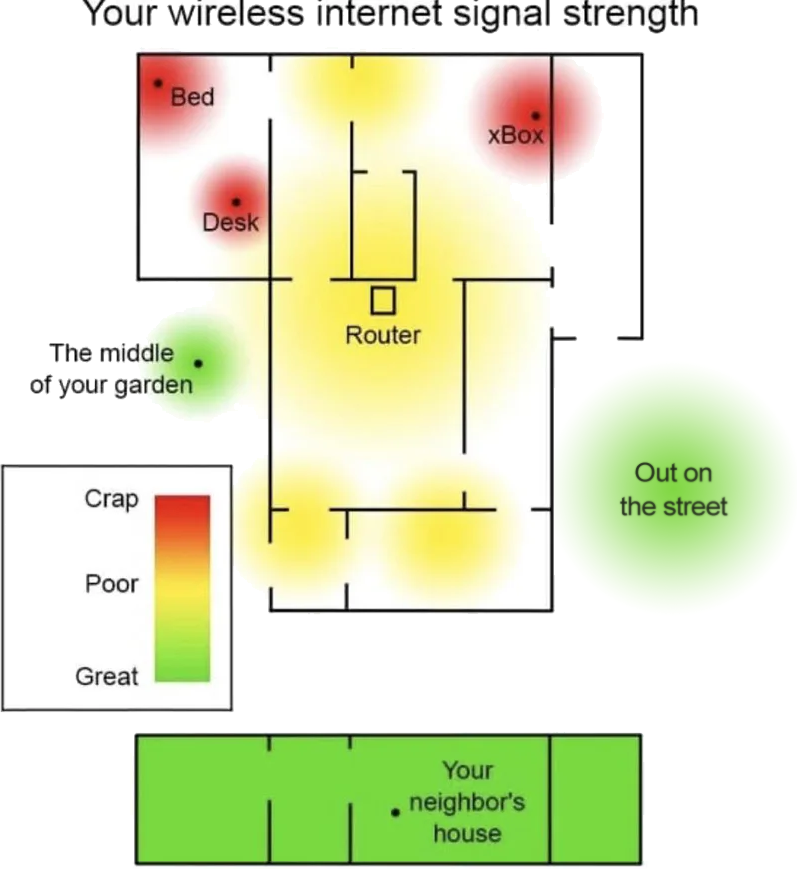
\includegraphics[scale=0.5]{img/wifi_signal.png}
    \decoRule
    \caption{You know it's true.}
    \label{fig:meme_wifi_signal}
\end{figure}

The formula also tells us that those how-tos suggesting to increase the maximum power transmission of the AP in order to get better performance are quite idiotic: in the EU there is a 100 mW limit on the AP power because of safety laws, so we cannot just change the Wi-Fi setup by telling it that it is located in a country outside the EU in order to make it use more power. Even if we did, this remains a bad suggestion, because even though we will get a better signal from the AP, the AP will not get more power from us: we might receive a better signal, but we would still be sending shit, the only result being a channel imbalance (also, forward and backward links might have different error probabilities, too).

Now, how far can the Wi-Fi signal travel before we can be reasonably sure that an attacker will not be able to decode it? Considering that the received power at the attacker should be low enough to be indistinguishable from a thermal noise, the answer is: further than we might think.

Every antenna on the field will receive some thermal noise due to the electromagnetic noise, which is always in the air either because of other devices or because of the ambient temperature (the heat). With normal equipment we easily think that we cannot receive our own Wi-Fi network signal from the outside, and thus that we are safe. However, if an attacker goes out there with low receiver losses equipment and a high gain antenna (usually a parabolic or a planar antenna), he/she will be able to easily decode our signal.

\vspace{0.5em}

\emph{Example} We could decode the Florence Careggi Hospital Wi-Fi from the UniFi Santa Marta offices with reasonably common equipment. Don't believe it? Give it a try.

\vspace{0.5em}

In conclusion, mind where the Wi-Fi devices are placed, because the signal travels a lot more than we think - and usually people forget about this.

%----------------------------------------------------------------------------------------

\section{Jamming}
\textbf{Radio jamming} is the deliberate blocking or interference with authorized wireless communications. Jammers work by transmitting radio signals that disrupt communications by decreasing the signal-to-noise ratio. The concept can be used in wireless data networks to disrupt information flow, and it is a common form of censorship in totalitarian countries, in order to prevent foreign radio stations in border areas from reaching the country.

Jamming is usually distinguished from interference that can occur due to device malfunctions or other accidental circumstances. Devices that simply cause interference are regulated differently. Unintentional jamming occurs when an operator transmits on a busy frequency without first checking whether it is in use, or without being able to hear stations using the frequency. Another form of unintentional jamming occurs when equipment accidentally radiates a signal, such as a cable television plant that emits on an aircraft emergency frequency.

Technically, jamming does not decrease the receiving power, but increases the noise received by the antenna (the miscellaneous loss $L_M$). Below a certain signal-to-noise ratio, the system will not be able to decode the signal, so a jammer needs to inject enough noise to overcome the intended signal.

Jamming can be either stupid or smart:

\begin{itemize}
    \item \textbf{stupid}: the jammer continuously injects noise in the channel;
    \item \textbf{smart}: the jammer waits for certain packets and injects spike noise when they arrive.
\end{itemize}

The stupid version could easily make the receiver realize that there is an attack undergoing, while with the smart one a jammer is much harder to find.

Generally, an attacker does not need to jam everything; they have to disturb the signal just enough to make it unusable. For example, in packets of 2000 bytes, modifying 10 bytes is sufficient to disrupt the data.

%----------------------

\subsubsection*{Countermeasures}
As the name implies, jamming is an attack that works for every type of wireless transmission, by increasing the miscellaneous loss $L_M$. It is always possible, and cannot be fought in any way that does not involve physically beating the jammer.

A simple way to (kinda) avoid it is to enlarge the spectrum of the receiver by using, for example, code division multiple access (CDMA), so that an attacker will have issues on blanketing the whole spectrum. The effectiveness of this method depends on the attacker's hardware though, and nowadays even CDMA is jammable.

Another way to avoid disturbances, either intentional or involuntary, is to frequently change the base frequency.

\vspace{0.5em}

\emph{Example} This technique is natively implemented by the Bluetooth protocol, which uses channel hopping. In order to jam a Bluetooth connection, an attacker has to either blanket all channels at once (stupid jamming), or to follow the hops and the packages - which is much harder, especially when they do not know how the channel hopping is performed.

%----------------------------------------------------------------------------------------

\section{Role of the MAC}
Moving from the physical layer up, there is the medium access control layer, which is very important. On wired networks this layer has very simple tasks.

\vspace{0.5em}

\emph{Example} For example, in the Aloha or Ethernet protocols, the MAC layer (together with the logical link control layer, see section \ref{sec:iso_osi}) only has to listen to the channel, see if somebody is transmitting, decide when to transmit, check if there have been collisions, schedule transmissions and other similar tasks, which are quite simple compared to its Wi-Fi counterpart.

\vspace{0.5em}

On Wi-Fi, and a number of other wireless system, the MAC layer has been bloated with other functions, including:

\begin{itemize}
    \item \textbf{access control}: deciding not only who is transmitting (and when), but also who \textit{can} and who \textit{cannot} transmit;
    \item \textbf{encryption}: something not really expected from this layer.
\end{itemize}

For these reason this layer is extremely important for the security of Wi-Fi systems.

%----------------------------------------------------------------------------------------

\section{Why is Wi-Fi so popular?}
This is actually a good question, because Wi-Fi is \textit{not} a good standard, but decent at most. It does not use channels efficiently, it is not energy efficient (it is the equivalent of a monster track with respect to an electric car; it eats power for breakfast) and its security is poor at best.

Radio coverage in the Wi-Fi protocol is not obvious: it can transmit at both 2,4 and 5 GHz, bandwidths dramatically impaired by walls and water. This, together with interference, kills performance, and is a serious problem. Moreover, Wi-Fi guarantees neither performance nor availability, not even at low rates.

Also, a number of Wi-Fi variants have been developed under the Wi-Fi brand even though they share practically nothing with the other kinds of Wi-Fi. An example is the 802.11ax standard, which uses a 6 GHz bandwidth.

A few reasons why Wi-Fi has become popular in spite of all this are:

\begin{itemize}
    \item it is \textbf{wireless}: nobody wants to have a spaghetti-like house or office, people love getting rid of cables;
    \item the hardware is \textbf{cheap}: like, \textit{really cheap}. Adding Wi-Fi capabilities to a device nowadays is almost free because of the efficient mass production methods that have been developed during the years;
    \item it is \textbf{everywhere}: since it is cheap, we find it even where we would not want it, quite literally;
    \item it is \textbf{fast} (sort of): despite sucking at energy saving and spectrum use, Wi-Fi works decently enough for users who only care about connection speed;
    \item it is \textbf{easy}: Wi-Fi devices are horribly simple to install and configure, making them perfect for the average user.
\end{itemize}

\begin{figure}[h]
    \centering
    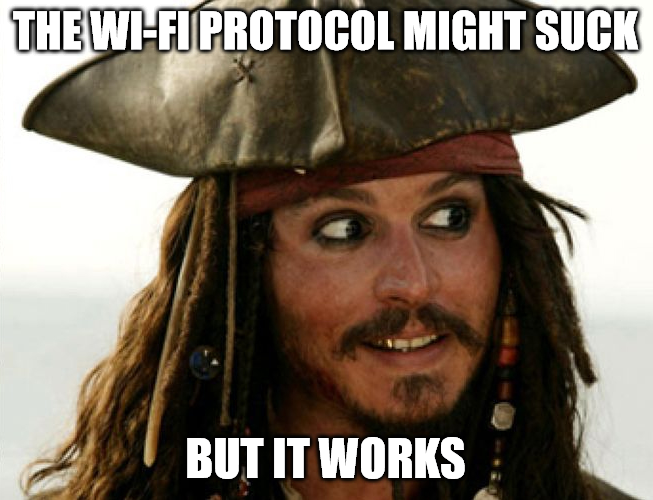
\includegraphics[scale=0.5]{img/wifi_sucks_meme.png}
    \decoRule
    \caption{It is hard to argue against this one.}
    \label{fig:wifi_sucks_meme}
\end{figure}

Still, never use Wi-Fi for any mission critical system because it might fail anytime.

%----------------------------------------------------------------------------------------

\section{Regulations}
Wi-Fi is regulated by the Wi-Fi Alliance, but it also follows \textbf{local} and \textbf{regional regulations}. These mostly differ in the frequency used, as they fall in the ISM band\footnote{ISM (Industrial, Scientific and Medical) bands are defined by the ITU (International Telecommunication Union) as industrial, scientific and medical applications of radio frequency energy: operation of equipment or appliances designed to generate and use locally radio frequency energy for industrial, scientific, medical, domestic or similar purposes, excluding applications in the field of telecommunications.} of portions of the spectrum not subject to licenses. The regulations say which bands can be used, what is the maximum transmitting power and for how long it can be used. Usually, devices have to follow a transmission-silence ratio, in order to allow other systems to use the same channel.

This is an overall good thing because everybody can install Wi-Fi freely, but it is also bad for the very same reason. The most used ISM bands are the following:

\begin{itemize}
    \item 868 MHz – 868,6 MHz (EU);
    \item 902 MHz – 928 MHz (US);
    \item 2,4 GHz – 2,5 GHz;
    \item 5,725 GHz – 5,875 GHz.
\end{itemize}

Wi-Fi practically never uses the first two bands. Mind that given the same power transmission, the lower the frequency the better the wall penetration of the signal.

%----------------------------------------------------------------------------------------

\section{Packets}
Wi-Fi packets come in three flavors:

\begin{itemize}
    \item \textbf{management}: everything that allows us to discover a nearby Wi-Fi network and join it ((de)authentication, (de)association, beacons, etc.);
    \item \textbf{control}:  what we would expect from a MAC system (RTS/CTS, ACK, etc.), or in other words what allows us to transmit on the channel without collisions, and to eventually know if our packet has been received or not;
    \item \textbf{data}: well, data (what did you expect?).
\end{itemize}
	
The first two types are mandatory and fundamental, but do not carry any data. Note that the only thing that is encrypted is the payload of data packets; headers are not encrypted - this is an important point, because it allows a number of attacks.

The missing encryption is a vulnerability by design (just design, not bad design) which shall be later discussed in detail.

%----------------------------------------------------------------------------------------

\section{RTS/CTS}
To put it simple, Wi-Fi does not encrypt everything that moves because some of the management frames (packets at MAC level) cannot be encoded or decoded if a device is not yet part of the network because of the missing key, and having previously negotiated one would mean killing the whole purpose of Wi-Fi.

Control frames, on the other hand, \textit{could} have been encrypted, because at control level a device is already part of the network. However, it has been decided to not encrypt them for compatibility reasons: when different networks coexist in the same ISM bands, it is a good idea to publicly declare what they are doing, so that they can decode what is being sent and act accordingly.

\vspace{0.5em}

\emph{Example} Using unencrypted control packets and data packets headers allows different Wi-Fi networks to decode each other's packets and avoid collisions. The same goes for different Wi-Fi versions, and even different standards (like Unlicensed LTE). Note that the complete opposite situation is valid for GSM, LTE and 5G, where management, control, data and everything else is encrypted because users physically posses a SIM card.

\vspace{0.5em}

\textbf{RTS/CTS} (Request To Send/Clear To Send) is the (optional) mechanism used by the Wi-Fi protocol to reduce frame collisions introduced by the hidden node problem (fig. \ref{fig:wifi_hidden_node}).

\begin{figure}[h]
    \centering
    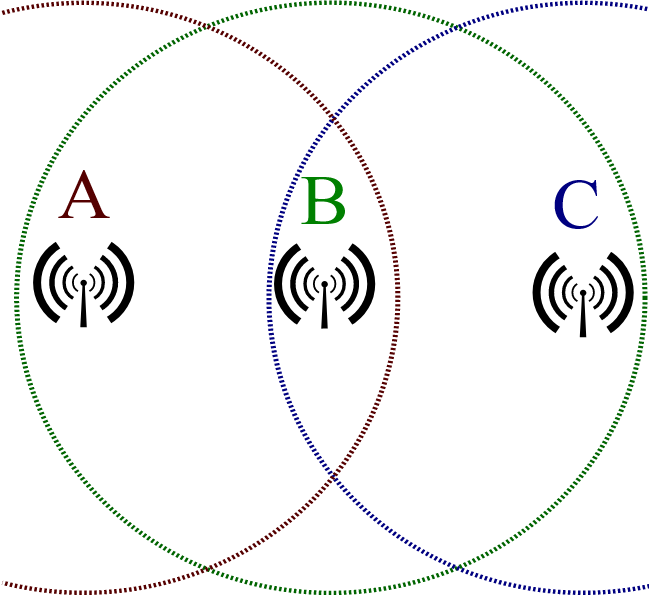
\includegraphics[scale=0.3]{img/wifi_hidden_node.png}
    \decoRule
    \caption{In one scenario, terminal A can communicate with access point B. C can also communicate with B. However, A and C cannot communicate with each other as they are out of range of each other, and if they transmit simultaneously, they prevent B from receiving any messages intended for it.}
    \label{fig:wifi_hidden_node}
\end{figure}

In order to solve this problem, control packets are sent to tell C that there is another device in B's range (A), and thus that it should be silent for a while so as to allow it (A) to send packets to B.

When sending data, terminal A does not send a packet straight to B; it first sends a short control packet, the \textbf{request to send} (RTS). Everybody can receive it, and whoever gets such a message knows that someone is trying to access the channel, so they will stay silent.

At this point B will send a \textbf{clear to send} (CTS) packet, which in turn will be received by every other terminal, including those who did not see the RTS. C will thus understand that somebody has reserved the channel, so it will wait and go in sleep mode.

Both these packets contain the \textbf{duration} of the packet to be transmitted, or in other words the time for which the channel is reserved by one terminal. This mechanism is incredibly powerful and useful for hidden terminals, even in different networks/protocols.

%-------------------------------------------

\subsection{RTS/CTS attacks}
\label{sec:wifi_rtc_cts_attacks}
As you might have already suspected, an attacker can do wonderful things with the RTS/CTS mechanism. The simplest one is to send fake RTSs with incredibly long durations, but could also be CTSs pretending that the access point is granting the channel to somebody else (who does not actually exist). By using very low power when doing this, it can generate CTSs only for a single, unsuspecting device, resulting in a very selective, jamming-like attack at MAC level. Again, there is no countermeasure against fake CTSs, because they are not encrypted and we cannot tell them apart from the regular ones. Reasonably, in case of a RTS/CTS attack we can try detecting if there are too many such messages in the network and raise a flag - although it would only mean that there \textit{might} be something strange and/or fishy, not that there is actually an attacker in the network (it could just be a PlayStation communicating with a controller).

The good news is that RTS/CTS is not often used by the Wi-Fi protocol, because in practice sending RTS/CTS messages takes too long. With the current Wi-Fi bitrates, normal data packets are much shorter than RTS/CTS exchanges, making them cumbersome: using them would make the channel bitrate drop very low. RTS/CTS is only needed when the probability to get packets corrupted by collisions is high enough, otherwise we can forget about it and just cross our fingers that collisions will not happen.

An interesting issue is that of the \textbf{minimum transmittable unit} (\textbf{MTU}). The Wi-Fi MTU is 2000 bytes, while for the Ethernet protocol is just 1500 bytes - so how is it possible to transmit packets from Wi-Fi over Ethernet? The answer is that the MTU is set by the Ethernet, so in all practical uses Wi-Fi uses packets much shorter than it should, and it resorts to longer packets only when two Wi-Fi stations communicate directly. Wi-Fi also implements \textbf{packet aggregation}, so we might see humongously large packets passing through. So all in all, it would be wrong to just say to our devices to ignore RTS/CTS messages; we simply do not use them very often, but the Wi-Fi Alliance clearly specifies that we must always be ready to obey them.

%----------------------------------------------------------------------------------------

\section{WEP}
\textbf{Wired Equivalent Privacy}, shortened by \textbf{WEP}, is a security algorithm for IEEE 802.11 wireless networks. Introduced as part of the original 802.11 standard ratified in 1997, its intention was to provide data confidentiality comparable to that of a traditional wired network: \textit{nomen omen}\footnote{\textit{The name is a sign}.}.

As soon as Wi-Fi has been created, it became immediately clear that sending data in plaintext was not a very good idea - not because a strong encryption for privacy was desired, but because of the coexistence of channels. Basically, developers did not want everybody to be able to listen to everybody else. WEP was introduced for this reason, and as the name implies it offered the same level of privacy as a cable: everybody on the same cable could listen to what others were transmitting. The goal was not introducing privacy between our devices and the AP, but only between different networks.

%-------------------------------------------

\subsection{Authentication and association}
Since WEP introduced encryption in Wi-Fi networks, it had to include a way to join and leave the network. In Wi-Fi, this requires two steps: \textbf{authentication} and \textbf{association}.

These two steps are different, and it is not to be taken for granted that we can authenticate \textit{and} associate to a network. Authentication only works if a device has been able to join the network, while association tells us if the device is on the network.

The reason for the existence of the association mechanism can be found in the fact that back in the days, access points were rather simple machines, very costly and with severe hardware limitations. They could only handle a limited number of devices at a time, so in order to manage networks with hundreds of hosts, association was needed so as to allow communication only to certain devices (the associated ones), while still keeping the others somewhat ready to transmit (the authenticated-only ones).

The phases that a device has to undergo in order to connect to a Wi-Fi network are as shown in figure \ref{fig:wep_states}.

\begin{figure}[h]
    \centering
    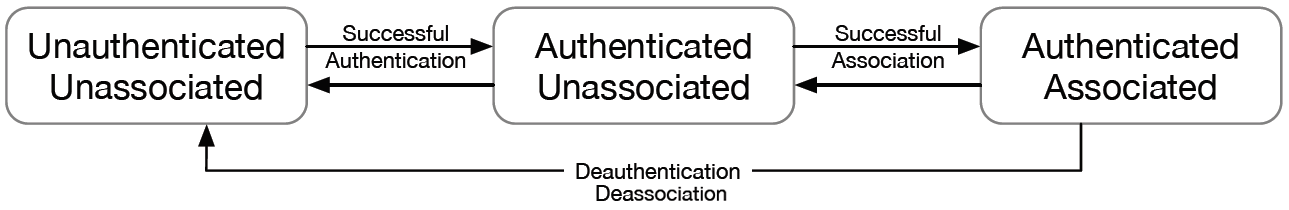
\includegraphics[scale=0.3]{img/wep_states.png}
    \decoRule
    \caption{WEP authentication and association phases.}
    \label{fig:wep_states}
\end{figure}

This process could have been done differently: instead of having three states, we could have had two states only (the first and the last ones) with a proper return code telling a device the reason why it cannot join the network at a given moment.

Three states, however, allow for faster switching between them: it is more efficient to kick somebody out from the association list and then let it back in, rather than kicking them from the network altogether. These steps are made through management frames, which are not encrypted, so an attacker could happily use forged packets to prevent someone from associating to a network. In fact, it is so easy that they would get bored very quickly (fig. \ref{fig:boring_wep_meme}).

\begin{figure}[h]
    \centering
    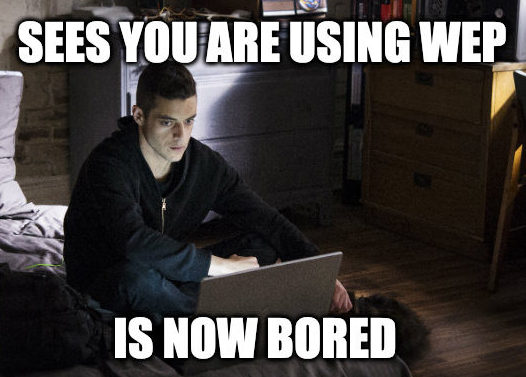
\includegraphics[scale=0.6]{img/boring_wep_meme.jpg}
    \decoRule
    \caption{Do not use WEP. Like IPv4, it's dead.}
    \label{fig:boring_wep_meme}
\end{figure}

It is important to understand that authentication and association are two separate concepts: one thing is saying \textit{"I know who you are"} and another is \textit{"you can do this or that"}. A device cannot communicate with other devices on the network if it has not successfully completed both the authentication and  association phases (all packets sent in any of the first two intermediate states will be discarded by the access point).

In other words, \textbf{authentication} demonstrates that we \textbf{know something}. It is executed in three steps:

\begin{enumerate}
    \item the device that wants to join the network sends an \textbf{authentication request};
    \item the access point replies with a \textbf{challenge};
    \item the device replies with an \textbf{encrypted challenge}.
\end{enumerate}

The challenge is encrypted with the secret, i.e. the network's password; the implicit assumption is that only the legitimate users know the secret.

Association at this point is nothing more than a simple two-way request-reply, only needed to make sure that the AP has enough available resources (IP addresses, places in the routing table and other physical assets).

%----------------------

\subsubsection*{What's the catch?}
The challenge in practice is nothing more than a random bunch of bytes, and so is the encrypted challenge, too (while the common knowledge is used as a symmetric key).

This whole process is not a real form of authentication; as devices who want to connect to the network, we are never identified as someone in particular. All we do is providing proof that we know something, a secret which is not even \textit{really} private (passwords can often be found in the most common and unsafe places). An AP will never know who is who, not even by looking at the MAC addresses since these can be spoofed (for legitimate reasons, too\footnote{Modern computers and phones often randomize their MAC address for both Wi-Fi and Bluetooth in order to avoid being tracked.}). And yes, you have probably already guessed that trusting a whole chain of users to keep their passwords private is a very bad idea, to say the least.

But the real problem with this challenge mechanism is that our (not so much) hypothetical attacker sees both the plaintext \textit{and} its encrypted form: it is a dramatic example of \textbf{information leakage}, as recovering the password with a brute force attack at this point is ridiculously easy.

%----------------------

\subsubsection*{More authentication and association attacks}
We already saw in figure \ref{fig:boring_wep_meme} how much WEP is boring for a decent \sout{hacker}\footnote{Oops.} attacker, so we are going to see now a few creative ways to perform a DoS (Denial of Service) attack on a Wi-Fi network - any Wi-Fi network, not just those with WEP encryption.

\begin{itemize}
    \item \textbf{de-association}: devices in the third phase (authenticated and associated) can be de-associated (or even de-authenticated) by an attacker pretending to be the AP; the terminal will constantly send association requests to the AP, while the AP itself will be confused about them because it still considers that device as associated. The result will be that not only the terminal under attack will be unable to communicate within the network, but also that the AP will collapse because of all the association requests from the device in question. Note that denial of service attacks can also be done during the second phase (authenticated/unassociated), but they are hard to execute because devices stay in this step only for a brief moment.
    \item \textbf{IP de-authentication}: in this case the victim is forced to repeat the authentication process, providing the attacker with another plaintext-encryption pair. By doing this repeatedly, the attacker gets enough information to retrieve the secret: while the probability of guessing the password from a single set of information is very slim, cryptoanalysis becomes possible when provided with more of them\footnote{One of the basic requirements of any form of cryptography is that from a clear text and its encrypted form an attacker should not be able to guess any of the bits of the key/secret/password, but since that is not universally true because they might be correlated, having more cyphered texts with the clear version yields better probabilities to guess the password. Each bit guessed right cuts the number of tries for a brute force attack in half: an important advantage.}.
\end{itemize}

An attacker does not even have to be connected to the network in order to perform these attacks, but only to forge a packet with the right source MAC address (which is sufficient, even though there are four MAC addresses in the Wi-Fi header) and the (unencrypted) management messages, so as to pretend being the AP. All the relevant parts are constantly sent in clear text management messages between the devices in the network and the AP.

Both attacks can be made automatic, and are easily successful. They not only prevent a device from connecting to the network, but also from finding out that there is an attacker, making us just think that the network is shit. They can be used for subsequent MitM (Man-in-the-Middle) attacks, too. These are vulnerabilities by design, the kind of which we cannot defend against.

The only possible countermeasure is to frequently change the SSID (Service Set Identifier, or the network's name) and the password in order to force an attacker who might have discovered the secret to find it again. However, periodically changing the secret means that we have to give a new password to all users, which is a PITA kind of process: users will send us to hell because they saved the passwords and SSIDs, and at the end of the day we will have a sign in the office with this information, or a piece of paper on the keyboard.

%----------------------------------------------------------------------------------------

\section{Wi-Fi frame}
\begin{figure}[h]
    \centering
    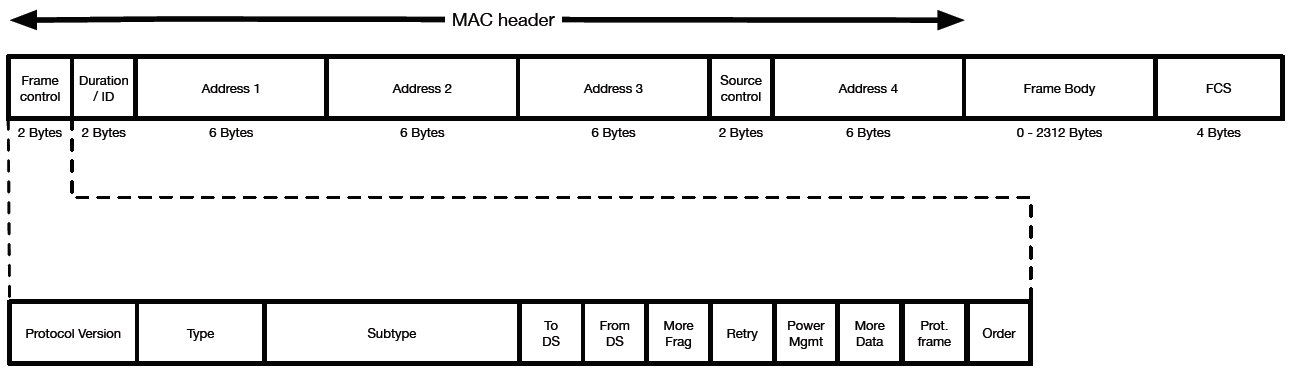
\includegraphics[scale=0.5]{img/wifi_frame.png}
    \decoRule
    \caption{Diagram of a Wi-Fi frame.}
    \label{fig:wifi_frame}
\end{figure}

The whole MAC header is never encrypted in Wi-Fi, not even in data messages. Management and control messages do not encrypt the frame's body, either (and of course, authentication and association are management frames). These frames, especially data frames, are transmitted using modulation and coding that might differ from what we are expecting. For this reason, when we have devices with different Wi-Fi standards in the same network (like 802.11b and 802.11n), the MAC header is transmitted at the rate of the lowest modulation encoding, meaning that the longer the header, the longer the time it will take to transmit the payload, too.

\vspace{0.5em}

\emph{Example} Suppose that we are using a very high modulation encoding, while the AP uses 802.11b, which by standard has a lower modulation encoding: the AP will not understand the most part of our headers, so we will have to transmit them at a lower modulation encoding.

\vspace{0.5em}

This is also the reason why we cannot trust how fast is our network, because what we know is probably the maximum rate, while in reality it could be much lower. In any case, we should \textit{always} be aware of the exact Wi-Fi version that we are using.

%----------------------------------------------------------------------------------------

\section{WEP encryption}
From the point of view of authentication methods, we probably already know that there are \textbf{WEP} and \textbf{WPA} (Wi-Fi Protected Access), both of which should never be used, then \textbf{WPA2}, the good one. There is also \textbf{WPA3}, but it is better if we just pretend that it does not exist.

A \textbf{stream cipher} is a symmetric key cipher where plaintext bits are combined with a pseudorandom cipher bit stream (a keystream). Each plaintext bit is encrypted one at a time with the corresponding bit of the keystream, resulting in a bit of the ciphertext stream. In practice, the combining operation is an exclusive OR (XOR). The stream cipher is used to encrypt authentication exchanges and data packets (payload only) in the WPA authentication methods. 

Generally speaking, the problem with data encryption (real data) is that we have to encrypt a finite number of bytes, not a real continuous stream, and often we also have to re-transmit them (because of errors, lost packets, etc.). Packets are not ordered, either: it is totally legitimate from the transmitter's point of view to send a packet while another has been lost, since layer 2 does not care about receipts (unlike TCP\footnote{TCP, on the other hand, does have a data stream, so a stream cipher on top of TCP could encrypt a whole message instead of single packets, allowing us to use a more performant and efficient cipher. TLS, for example, being on top of TCP, can leverage the TCP stream nature. On the contrary, BTLS (the TLS equivalent for UDP) cannot do this, because UDP is not a stream protocol.}, which is however layer 4). This makes the use of stream ciphers on single packets (rather than on the whole data stream) sub-optimal, since it would resemble more a block cipher\footnote{The downside of block ciphers, which encrypt different blocks of bytes with the same key (like the Feistel algorithm), is that since each block is independent, all blocks have the same confusion and diffusion, thus making this encryption method less effective than stream ciphers.}.

OTP, on the other hand, requires an encryption stream as long as the message; basically, instead of splitting the message into blocks, it encrypts it whole. Still, we could encrypt the message one byte at a time by maintaining the state of the previous byte.

%-------------------------------------------

\subsection{OTP rethinked}
The Wi-Fi stream cipher is very similar to the OTP. In OTP we need a message and a randomly generated key (a secret) $K$ as long as the message:

\begin{equation}
\label{eq:wifi_otp}
        C = M \oplus K
\end{equation}

In Wi-Fi, the secret shared with the access point is not the same $K$ as in equation \ref{eq:wifi_otp}; it is used instead as \textbf{input }to a \textbf{PRNG} (Pseudo-Random Number Generator), a black box\footnote{Not that black in reality because usually we know how it works.} which, given an input, generates a stream of random bits or bytes.

Any PRNG will generate the same random number (not so random at this point) if given the same initialization state (the seed). We need thus a cryptographically strong seed, something with \textbf{no correlation} between the output bits, nor between bit couples, triplets, any multiples, and not only at bit level, but also of byte. Every single bit, regardless of its position in the byte that has been generated, should have exactly 50\% probability of being 0 or 1 (statistical independence).

PRNGs are nothing more than algorithms, and so they have internal states; at one point their state will return to the initial one, after which the secrets will repeat themselves: this is called a \textbf{cycle length}, and in order to have a good PRNG it has to be as long as possible. In practice, the minimum cycle should be longer than the maximum transmittable packet (64.000 bits in Wi-Fi).

Some PRNGs are sensitive to certain numbers (like odd or even numbers), meaning that the output generated by sensitive seeds will contain significant correlations. For this reason, we must know well how our PRNG works, and be aware that we might have to blacklist some inputs. Generally, initializing it to the time of the day or to very large numbers is not very effective.

Now, suppose that we have a good PRNG, and that we can have a key - a random seed - that can be easily given to the system and is not the same for every packet (otherwise every packet would be encrypted with the same sequence, and the whole thing would be useless). How do we change the seed for every packet?

%----------------------

\subsubsection{Payload encryption}

\begin{figure}[h]
    \centering
    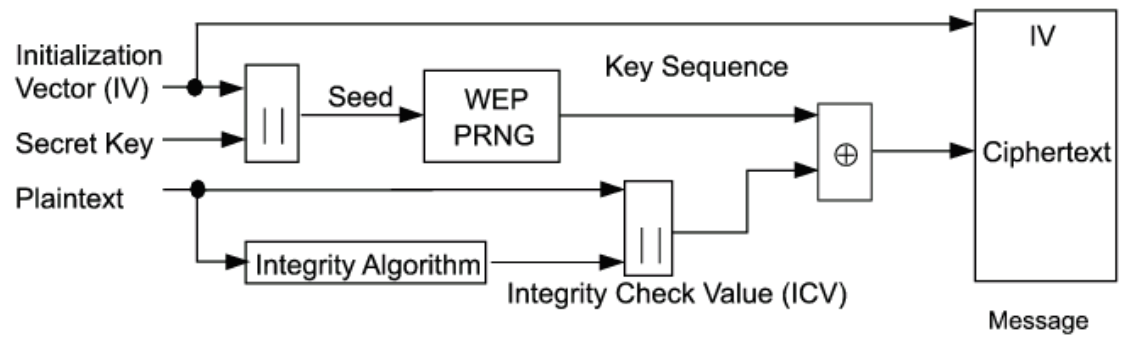
\includegraphics[scale=0.5]{img/wifi_wep_encryption.png}
    \decoRule
    \caption{WEP encryption process.}
    \label{fig:wifi_wep_encryption}
\end{figure}

\begin{figure}[h]
    \centering
    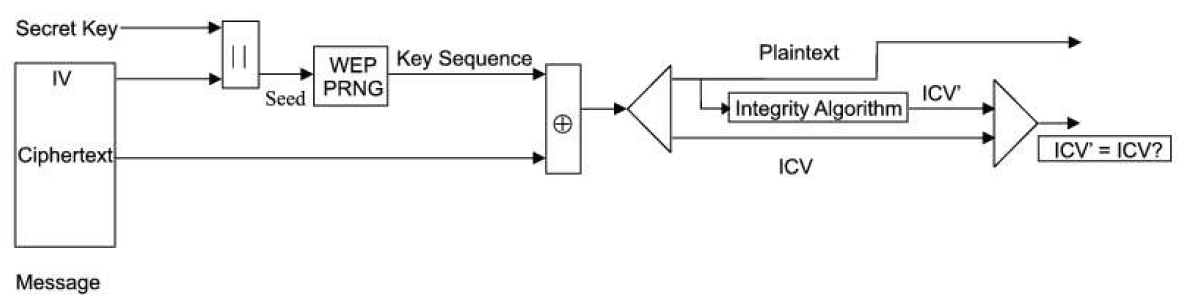
\includegraphics[scale=0.45]{img/wifi_wep_decryption.png}
    \decoRule
    \caption{WEP decryption process.}
    \label{fig:wifi_wep_decryption}
\end{figure}

In order to encrypt data packets payloads, WEP uses the Wi-Fi password to get the secret key, which is a simple hash of the password itself (otherwise it would not be random enough, since it would probably use letters which in turn could be predictable because of ASCII codes). So, the encryption procedure for WEP is as follows:

\begin{enumerate}
    \item hash the Wi-Fi network password to get the secret (key);
    \item concatenate the key with the \textbf{IV} (Initialization Vector, a fixed-size input to a cryptographic algorithm typically required to be random or pseudo-random) to get the PRNG seed;
    \item use the PRNG to generate a random stream of bytes;
    \item concatenate the plaintext with the the \textbf{ICV} (Integrity Check Value, a hash of the plaintext);
    \item XOR the bits from step 4 with the random stream from step 3;
    \item add the IV at the beginning of the ciphered message.
\end{enumerate}

The secret in WEP is 40 bits long, while the IV is 24 bits long; by standard, the PRNG is \textbf{RC4}\footnote{In cryptography, RC4 (Rivest Cipher 4) is a stream cipher, remarkable for its simplicity and speed in software.} and the ICV is \textbf{CRC32}\footnote{A cyclic redundancy check (CRC) is an error-detecting code commonly used in digital networks to detect accidental changes to raw data. The 32 in CRC32 indicates that it is 32 bits long.}. Everything seems good, right? Bad news: all this is plain shit. There really are no other words for it: it is a pile of gigantic crap.

First of all, 40 bits for a secret is way too short: no matter how long or complex we make our password, WEP will always encode it in a hash of 5 bytes; considering that hashes have a significant probability of collision, too, 5 bytes really are not enough.

Second: 24 bits in the IV means that even if we used this vector in a smart way (for example by ordering the packets), after $2^{24}$ packets it would repeat itself, and if we repeat it without changing the secret key we will get the same secret. $2^{24}$ is too small a number: 16+ million packets are \textit{nothing} in a networking system (it is a good example of \textit{very} bad design).

\vspace{0.5em}

\emph{Example} Suppose we have a 1 Gb/s connection. If we divide 1 Gb/s by 8 so as to get bytes, then calculate the number of packets sent per second, we can easily see that in order to send $2^{24}$ packets we only need \textit{5 hours}.

\vspace{0.5em}

Third: the RC4 PRNG had been recently designed and was not tested sufficiently when the standard was created. The result is that the standard needs a specific PRNG which now has been proven to not be cryptographically strong, as it has correlations between the key and the seed (basically, by knowing the randomly generated sequence one could derive the key or part of it).

Last but not least, CRC32 is fantastic, but it is a simple integrity check value, meaning that it is there only to allow to check whether the packet has been received correctly. It is not a hash value, so it does not have either confusion or diffusion, making it very easy for an attacker to guess it.

So yes, all these four things have been made in the wrongest possible way.

\textbf{WEP decryption} is very similar to encryption, so there is not much to say about it: having the secret key and the IV (which we got from the packet), we regenerate the seed, get the key sequence, decrypt the cyphered text and then check the ICV.

%-------------------------------------------

\subsection{Blind attacks}
We might think that we are safe because the attacker only sees the ciphered text, and that it would have to have a clear text, too, in order to recover the stream and expose the correlation in the RC4 PRNG. Well, no: there is one part where we are actually \textbf{transmitting the clear text \textit{and} its encryption}, which is during authentication. An attacker can simply de-authenticate somebody, allow them to re-authenticate, and get the plaintext and the cyphered text.

\begin{figure}[h]
    \centering
    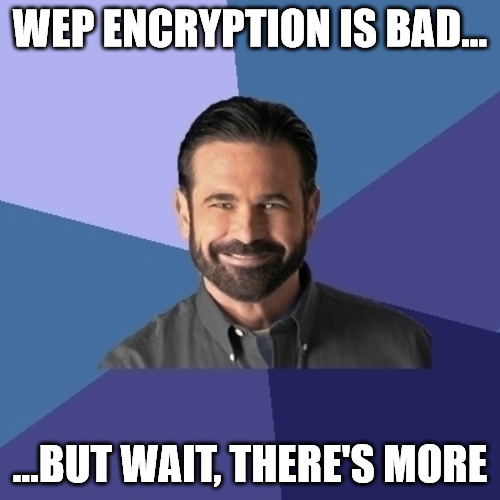
\includegraphics[scale=0.5]{img/meme_wep_wait_theres_more.png}
    \decoRule
    \caption{Did you seriously think that we were finished?}
    \label{fig:meme_wep_wait_theres_more}
\end{figure}

\textit{But wait, there's more} (fig. \ref{fig:meme_wep_wait_theres_more}): \textbf{CRC32 is even worse}, because its code is publicly available. It is fast, but it is also linear and easily invertible\footnote{From the point of view of security, linearity is the best thing that an attacker could ever wish for.}. It is nothing more than a XOR and shift.

Normally, in order to modify a message, we have to decode it and encode it again after having modified it. In a \textbf{blind attack} we do \textit{not} need to decode everything: we just have to \textbf{bitflip} a part of it. For example, if we want to change a "yes" to a "no" we just have to bitflip the bits than contain the "yes" part. In binary protocols we \textit{know} the position of the bits and their meaning, so using this same idea we can change any number into any other number.

How do we bitflip a message? If we know the clear text, we take the message and we just use a XOR with the 1s in the locations where the bitflipping should occur (and the 0s in the parts where the message should not be changed).

We can do the same to an encrypted message if the encryption has been done with a simple XOR (like WEP's stream cipher). The CRC could, in theory, prevent us from doing so, but since the CRC is based on the message, which in turn is nothing more than the IV concatenated to the actual data to be sent ($M_p$), we can split the key $K$ in two parts having the same size, $K_p$ and $K_c$, as shown in equation \ref{eq:crc32} (where $C$ is the encrypted message, and $M = M_p \parallel \operatorname{CRC}(M_p)$ is the message with CRC):

\begin{equation}
\label{eq:crc32}
\begin{aligned}
    C =& K \oplus M\\
    =& (K_p \parallel K_c)  \oplus (M_p \parallel \operatorname{CRC}(M_p))\\
    =& (K_p \oplus M_p) \parallel (K_c \oplus \operatorname{CRC}(M_p))\\
    =& C_p \parallel C_c
\end{aligned}
\end{equation}

The lengths of the CRC and of $M_p$ are known; due to linearity, this operation is equal to $K_p \oplus M_p$ concatenated to $K_c \oplus \operatorname{CRC}(M_p)$ (second line of equation \ref{eq:crc32}). If we want to modify some bits of the message, we just have to calculate $M'_p = M_p \oplus d$ (where $d$ is a message as long as $M_p$ made of all zeros, except for the 1s put where we want the original bits to be flipped).

\begin{equation}
\label{eq:crc32_2}
\begin{aligned}
    C' =& K \oplus (M'_p \parallel \operatorname{CRC} (M'_p) \\
    =& (K_p \oplus M_p \oplus d) \parallel (K_c \oplus \operatorname{CRC}(M_p \oplus d)) \\
    =& (K_p \oplus M_p \oplus d) \parallel (K_c \oplus \operatorname{CRC}(M_p) \oplus \operatorname{CRC} (d)) \\
    =& (C_p \oplus d) \parallel (C_c \oplus  \operatorname{CRC}(d))
    \end{aligned}
\end{equation}

Theoretically, we cannot calculate $M'_p$ directly because we do not know either $M_p$ nor $\operatorname{CRC}(M'_p)$ (see the second line of equation \ref{eq:crc32_2}), but thanks to linearity all these relations are known: $C_p$ and $C_c$ can be sniffed, $d$ is ours, and the CRC can be calculated, so at the end of the day we can bitflip any message without even decrypting it. We only have to guess what kind of packet has been sent, and if it is a bit stream we can change it to anything.

%-------------------------------------------

\subsection{KoreK's chop-chop attack}
Do we really need the secret key in order to decrypt a message? Spoiler alert: we don't.

Let us do some math: the variable part in the WEP seed is the IV, which has over 16 billion possibilities; typically, a Wi-Fi message (packet) is about 2.300 bytes (we could also have jumbo or smaller frames, these ones if we are attached to Ethernet): 40 GB of data would be enough to store a sample of every possible keystream.

We can therefore collect all packets going into the Wi-Fi network, trash those with the same IV and only store those with different IVs; after a while we will have a sample of all the possible key streams (IVs), which will allow us to use the Wi-Fi without even knowing the secret key, since what we really need is not the key itself, but the association between the IV and the keystream relative to that IV (assuming that the secret did not change in the meantime). Of course, we will have to extract the IVs from the rest of the bytes in each packet.

In order to extract the actual keystream, we have two possibilities:

\begin{itemize}
    \item \textbf{de-authentication attack}: we get a small keystream fragment, which we will have to enlarge in order to use (we need enough bytes to send and decode packets);
    \item \textbf{KoreK’s chop-chop attack}\footnote{\url{http://www.netstumbler.org/unix-linux/
chopchop-experimental-wep-attacks-t12489.html}}: by exploiting periodic fixed-length packets\footnote{These packets are address requests and replies, thus they have a well-known structure.}, typical of DHCP environments (or in other words, of practically all Wi-Fi networks), we get some bytes of the keystream from them. However, in those packets some bytes are fixed while others are variable, meaning that we will collect something that will be with great probability part of the keystream, but without real certainty. At this point though we will be able to reconstruct what we do not know by using KoreK's chop-chop attack.
\end{itemize}

Everybody deemed impossible this kind of attack, until someone showed on a forum that it was very possible indeed. \textbf{KoreK’s chop-chop attack} has two different versions; we will see the original one, since the other is exactly its opposite.

The main assumption is that we \textbf{do not know anything} about the packet. We shall explain how this attack works with the following example.

\vspace{0.5em}

\emph{Example} Let us suppose that we have sniffed a packet with some random data as shown in table \ref{tab:korek_1}, from $D_0$ to $D_5$ (these are bytes; note that there can be as many $D$s as we want), and a CRC from $J_3$ to $J_0$, encrypted with the keystream from $K_0$ to $K_9$. The result is an encrypted packet that goes from $S_1$ to $S_9$. Mind that we only know the part from $S_1$ to $S_9$; we do not know anything else yet.

\begin{table}[h]
    \centering
    \begin{tabular}{@{}llllll|llll@{}}
        \multicolumn{6}{c}{Data} & \multicolumn{4}{|c}{CRC}\\
        \midrule
        $D_0$ & $D_1$ & $D_2$ & $D_3$ & $D_4$ & $D_5$ & $J_3$ & $J_2$ & $J_1$ & $J_0$\\
        $\oplus$ & $\oplus$ & $\oplus$ & $\oplus$ & $\oplus$ & $\oplus$ & $\oplus$ & $\oplus$ & $\oplus$ & $\oplus$\\
        $K_0$ & $K_1$ & $K_2$ & $K_3$ & $K_4$ & $K_5$ & $K_6$ & $K_7$ & $K_8$ & $K_9$\\
        \midrule
        $S_0$ & $S_1$ & $S_2$ & $S_3$ & $S_4$ & $S_5$ & $S_6$ & $S_7$ & $S_8$ & $S_9$
    \end{tabular}
        \decoRule
        \caption{KoreK’s chop-chop attack, first step.}
        \label{tab:korek_1}
\end{table}

\begin{table}[h]
    \centering
    \begin{tabular}{@{}lllll|llll@{}}
        \multicolumn{5}{c}{DATA} & \multicolumn{4}{|c}{CRC}\\
        \midrule
        $D_0$ & $D_1$ & $D_2$ & $D_3$ & $D_4$ & $I_3$ & $I_2$ & $I_1$ & $I_0$\\
        $\oplus$ & $\oplus$ & $\oplus$ & $\oplus$ & $\oplus$ & $\oplus$ & $\oplus$ & $\oplus$ & $\oplus$\\
        $K_0$ & $K_1$ & $K_2$ & $K_3$ & $K_4$ & $K_5$ & $K_6$ & $K_7$ & $K_8$\\
        \midrule
        $S_0$ & $S_1$ & $S_2$ & $S_3$ & $S_4$ & $R_5$ & $R_6$ & $R_7$ & $R_8$
    \end{tabular}
        \decoRule
        \caption{KoreK’s chop-chop attack, second step.}
        \label{tab:korek_2}
\end{table}

We build now another packet, one that is \textbf{one byte shorter} than the previous one. Suppose that we want to send the bytes from $D_0$ to $D_4$ (killing $D_5$), as shown in table \ref{tab:korek_2}. This new packet will have another CRC, from $I_3$ to $I_0$, which will be different from $J_3$ to $J_0$, but we suppose to encrypt this packet with the \textbf{same keystream}, from $K_0$ to $K_9$: since it will be only one byte shorter, we only kill $K_9$.

Some parts of the new packet will be identical to the old one, i.e. the bytes from $S_0$ to $S_4$; the rest of the bytes are different: $R_5$ to $R_8$ have nothing in common with $S_5$ to $S_9$.

One could ask \textit{“how many attempts the attacker has to do in order to find out the right bytes?”} The dumb answer would be $2^{32}$ (because there are $8 \cdot 4$ bytes $= 32$ bits).

Of course, it would not be dumb if there was another, better answer. If we do some math, though, we find out that there is a \textbf{relationship} between $S_5$ to $S_9$ and $R_5$ to $R_8$, dependent on a number between $0$ and $255$ (because it depends on just one byte). So in practice we can obtain the second packet from the first by just guessing the value of this number.

We can continue by continuously changing one number until we get the bytes from $R_5$ to $R_8$. The number that we have to find out is $D_5$, meaning that all the relationships between $S_5 -  S_9$, $R_5 - R_8$ and everything else can be expressed in terms of $D_5$. When we find the right number, $D_5$, we can also calculate $K_5$, which is one byte of the keystream. We will also know $R_5$, and we will be able to repeat the process by cutting out $D_4$: everything shifts and we discover $K_4$, and then $K_3$, $K_2$, $K_1$ and $K_0$. At this point we have all $K$s from $K_0$ to $K_4$, so we can continue with the opposite operation (the reverse version of the chop-chop attack, which uses a packet one byte longer) for the remaining part, so that in the end we will get the whole keystream.

\vspace{0.5em}

There is only one thing left: who will tell us that we got the number right? Why, the access point will! It is only a matter of sending the packet to the AP with the numbers which we found, and it will send us an ACK if the packet has been received successfully. It does not even matter if the packet’s contents make sense for the IP layer, we only need the confirmation that we got the right keystream. How many tries do we have to do? With 128 tries we can find one byte; by doing some math, we can build up the keystream in practically no time.

There is another dramatic consequence of this, because once we got one keystream done, we do not have to redo everything for every other keystream (the 16 billion that we mentioned in the beginning). We only need to ping the AP. Once we got the first keystream, we send a ping message with it. The ping is an ICMP echo, which gets us back an ICMP reply encrypted with a different IV. The ICMP echo reply is identical to the one we sent except for one bit, which we know exactly where to find, so calculating every other keystream is a joke.

%-------------------------------------------

\subsection{Fluhrer, Mantin and Shamir attack}
But wait, there's more. \textit{Again.}

In 2001 \textbf{Fluhrer, Mantin and Shamir} published the cryptoanalysis of RC4 (which already was a standard), showing that it was \textit{not} a good pseudo-random number generator as it allowed to decrypt the Wi-Fi secret with a sufficiently large number of sniffed packets. While the KoreK chop-chop attack is an active attack, so we can somehow defend ourselves by implementing a traffic analyzer which can see if there are too many strange packets and raise an alarm, attacks on RC4 are purely \textbf{passive}. They are not even a kind of brute force attacks, but are possible due to the limitations of RC4.

The first attack discovered by these researchers was pretty complicated, because it required a large number of packets and took quite some time to do, so we were safe if the network was practically silent (since it depended on the amount of data that was being sent). Unfortunately, in 2005 \textbf{Klein} found more correlations in RC4, and in 2007 \textbf{Tews, Pychkine and Weinmann} extended further the attack making it enough to collect 85.000 packets to decode a 104-bit long secret (longer than the original WEP model; see figure \ref{fig:meme_thanos_wep}).

\begin{figure}[h]
    \centering
    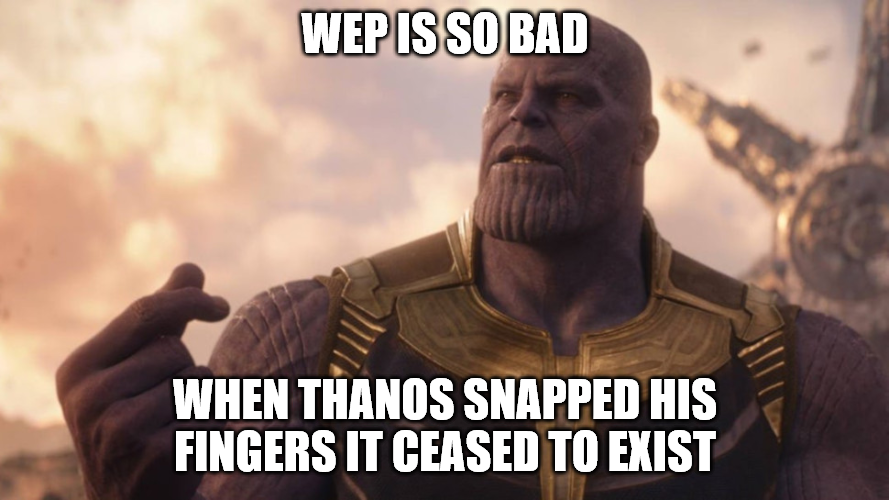
\includegraphics[scale=0.5]{img/meme_thanos_wep.png}
    \decoRule
    \caption{Shit got real: finding a WEP password and being able to ravage a Wi-Fi network was like the snap of a finger (85.000 packets in a normal Wi-Fi network are nothing).}
    \label{fig:meme_thanos_wep}
\end{figure}
 
There are some initialization vectors that expose directly some bits of the password, halving again the number of tries. In order to fix these issues there have been some proposals:

\begin{itemize}
	\item use a \textbf{larger IV}, making a chop-chop attack more difficult (actually ineffective, since finding successive keystreams after the first one is still linear, and anything good from a security point of view should exponentially raise the difficulty; moreover it would not solve the problems with RC4);
	\item \textbf{ditch RC4}: it is clearly bugged.
\end{itemize}

%----------------------------------------------------------------------------------------

\section{WPA}
Although slowly, we finally transitioned to \textbf{WPA} (\textbf{Wi-Fi Protected Access}), because WEP had way too many problems. WPA comes in three versions: \textbf{WPA}, \textbf{WPA2} and \textbf{WPA3}, but they all share the same architecture.

\begin{figure}[h]
    \centering
    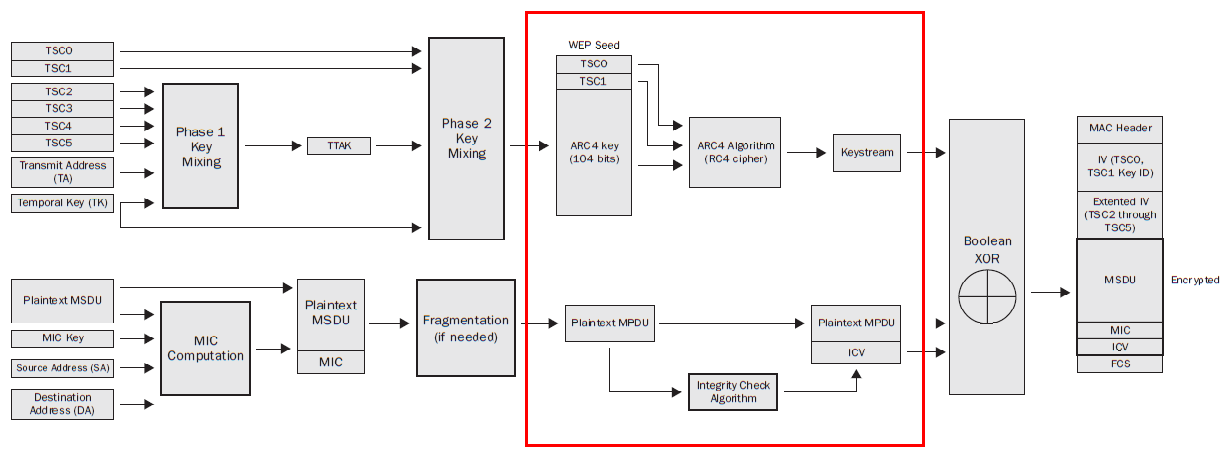
\includegraphics[scale=0.5]{img/wpa_encryption.png}
    \decoRule
    \caption{WPA encryption diagram; the part in red is the original WEP algorithm.}
    \label{fig:wpa_encryption}
\end{figure}

We can immediately see from figure \ref{fig:wpa_encryption} that it is far more complicated than WEP, although it still contains something that we really do not like: RC4.

%-------------------------------------------

\subsection{RC4 in WPA}
Why RC4? Well, it was mandatory: networks cards were bulky and costly at the time, RC4 was embedded in the hardware, and if we told the producers that they had to trash their products, they would not have said not very nice things to us.

The question was how to \textbf{reuse} the old hardware within a better system. The solution was to devise a new method that in most cases could have been applied as a firmware update, and at the same time make it more complicated so as to mitigate the RC4 bugs.

What changes in WPA is that the PRNG seed is not only made by the IV and the secret, but consists of a key (now 128 bits long) and some more data (TSC0, TSC1, TSC2, TSC4, TSC5, a transmit address TA and a temporary key TK). This new security protocol is called \textbf{TKIP} (\textbf{Temporal Key Integrity Protocol}).

TSC0, TSC1, TSC2, TSC4 and TSC5 (TKIP Sequence Counter) are simple counters, while TA (Transmit Address) is our own address. Together with the temporary key and the TA they are mixed together in two phases to generate a RC4 input. The integrity check algorithm is also still there, but at this point we have a different sort of checksum, the \textbf{MIC} (Message Integrity Check, which like the CRC only guarantees \textit{integrity}), but it is encrypted with another key, the MIC key, before sending the whole thing. This looked like a decent system, and it actually was one for years.
 
\textbf{WPA2} only switched from TKIP to \textbf{CCMP}\footnote{CCM mode Protocol, or Counter Mode Cipher Block Chaining Message Authentication Code Protocol is an enhanced data cryptographic encapsulation mechanism designed for data confidentiality.} and \textbf{AES} (Advanced Encryption Standard), which basically changed the RC4 and the Integrity Check Algorithm parts (the new algorithms for encryption).

The interesting part about WPA2 is that by changing altogether the encryption and integrity check we could get a simpler scheme. This means than WPA2 is a little faster than WPA.

%-------------------------------------------

\subsection{WPA security}
Before 2018 some attacks on WPA and WPA2 had already been found, such as a variant of the chop-chop attack that was still possible and allowed the attacker to build a dictionary of the keystreams; however, there were a lot keystreams, so basically the amount of data that he/she would have to store would have been extremely large.
 
In 2018 \textbf{KRACK} was found; it was an attack that used the 4-way authentication handshake to discover the temporary password. 
 
We have already seen that while in WEP there was a secret key which was a hash of the common secret, WPA and WPA2 use a \textbf{temporary key}. This temporary key is private to the user and the AP, and is negotiated during the authentication and authorization phases. So while in WEP every user could decode the packets of every other user in the network, in WPA this is not possible because every user has its own temporary key. Clearly, by finding it out an attacker is able to decode all packets of a certain user – and this is exactly what KRACK managed to do.
 
For this reason, KRACK is a particularly bad attack, because the WPA/WPA2 4-way handshake is embedded in these standards, so it exploits a vulnerability by bad design which cannot be fixed.

%----------------------

\subsubsection*{WPA 3}
When KRACK was discovered, the Wi-Fi Alliance forget everything that they had done wrongly in the past and… did it again. Basically, if they would have had to choose how to screw up properly, they probably would not have done a worse job in screwing up.

They hurriedly created a new version of WPA, \textbf{WPA3}, and they did it mainly behind closed doors with a rush in decisions about what to use as encryption and cyphering methods, and finally they used a new handshake method named \textbf{Dragonfly}. It was so new that nobody had heard about it before. And as soon it was out, someone found an attack, \textbf{Dragonblood}, which made Drangonfly even worse than WPA2.

At the end of the day, we will probably never see WPA3 in the wild. Security is not better, its implementation is a nightmare and producers would have to change the firmware in order to offer it to their users. The Wi-Fi Alliance should have first make a proposal and then let mathematicians and white hats play with it, just in case they forgot something, because mistakes in design should always be avoided. Generally speaking, we need to have things \textbf{tested out} by somebody else for enough time, and standards have to be \textbf{publicly discussed}. History tells us that anything done behind closed doors will be bad.